\section{Configuration in Magnolia CMS}
By means of the \emp{Location Framework} and \emph{MVP} pattern which were
described before we have defined a foundation for an abstract loosely coupled
system which is capable loading, rendering and disposing some components.
Adding a new functionality in such a system would only require to
implement its logic and to add the proper mapping, so the system would load the
component on demand. However, the end developer should not be required to change
the source files or mapping configuration manually. Instead there should be an
interface by means of which the developer would interact with the system and
alter its state. In the current section we will analyze the approach of a
high-level definition mechanism used in Magnolia 5.0.

Configuration mechanism is an essential feature of many software products. It
enhances the flexibility and extensibility in the sense that the person without
deep knowledge of the system internals can alter its behavior, re-arrange and
customize its parts. 

Magnolia CMS is also configurable by means of XML. Each module has an XML
descriptor containing all the properties needed for its description. An example
of a configurable component could be a registry of the forms with fields which
would be represented with a set of XML nodes with properties and sub-nodes for
fields types, captions, default values, validators etc. 

Most of Magnolia CMS configuration files are kept within \emph{config}
workspace. Displaying this workspace in a form of editable tree would allow the
user to modify the components visually in real time as long as the system
instantly reacts on those changes.
There are several techniques in Magnolia CMS that are used for applying the
configuration. The main two concepts are \emph{observation} and \emph{Node2Bean}.

\paragraph{Observation} is a feature of JCR that allows for subscribing to the
changes in a workspace. Observing applications can monitor and react on those
changes whenever the persistent operation is made in JCR. This feature has found
various ways of applications in Magnolia CMS. For instance, one of the most
important ways is the foundation for the factory-based [TODO: consider factory
appendix] structures: some sort of bindings are stored in a workspace in a form
of the registry which is later used in the factory to produce the actual objects.

\paragraph{Node2Bean} is used to convert the JCR nodes into the Java objects. 

By means of Java Reflection (introspection mechanism) Node2Bean binds the the
fields of a Java Bean to the corresponding configuration properties (if such are
available) through the bean's "setter" and "adder" methods. Node2Bean can
support all possible data types:
\begin{itemize}
  \item Simple data types like \texttt{String, int, long, float, double, boolean}.
  \item Collections with String values or other data types by specifying a class property.
  \item Maps with keys and values as Strings or other data types by specifying a class property.
  \item Complex classes can be mapped with Node2Bean by means of the sub-nodes
  which follow the same rules and restrictions.
\end{itemize}

Let us consider an example of using Node2Bean:

\begin{figure}[H]
	\centering
	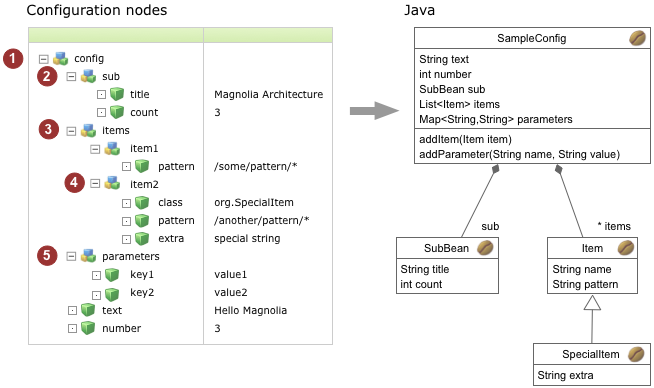
\includegraphics[width=\textwidth]{node_to_bean.png}
	\caption{Node2Bean mapping example}
	\label{fig:node2bean}
\end{figure}

Numbered items:

\begin{itemize}
  \item config: Entry point of the transformation. In the module descriptor
  \texttt{SampleConfig} class is used. Set text and number properties.
  \item sub: Sub bean. The class is determined using reflection if it is not
  explicitly defined.
  \item items: Collection. The corresponding add method is used to determine the
  class and populate the collection if existing.
  \item item2: Special item with its own class and additional properties.
  \item parameters: Collection of key-value pairs.
\end{itemize}
